\documentclass[10pt, titlepage]{article}

\usepackage[margin=1in]{geometry}
\usepackage{fancyhdr}
\usepackage{amsfonts}
\usepackage{amsmath}
\usepackage{amssymb}
\usepackage{booktabs}
%\usepackage{tikz}
\usepackage{float}
\usepackage{bm}
\usepackage{pgfplots}


\title{\normalsize PLUS Session Worksheet \\[1em] \Large \textit{MATH 1554:} Linear Algebra}
\author{\textit{Covering Sections:} 1.5}
\date{Fall 2023}

% ------- Set up header -------
\renewcommand{\sectionmark}[1]{\markright{#1}} % from https://tex.stackexchange.com/a/317393/227665
\pagestyle{fancy}
\fancyhead[L]{A. M., Fall 2023}
\fancyhead[C]{\textit{\nouppercase{\rightmark}}}
% \fancyhead[C]{\textit{(6.1), (6.2), \& (6.3)}}
\fancyhead[R]{\textbf{\thepage}}
% -------------------------------------------------------

% ------- Set up question environment -------
\newcounter{question}
\setcounter{question}{1}
\newenvironment{newquestion}
{
	\noindent\textbf{Question \thequestion}
}
{
\stepcounter{question}
\par
}
% -------------------------------------------------------

% ------- Set up Main Idea box environment -------
\newcounter{mainideas}
\setcounter{mainideas}{1}
\newcommand{\mainidea}{\textbf{Main Idea \#\themainideas \stepcounter{mainideas}}}
\setlength\fboxsep{1em}
%\newcommand{\midea}[2]{\begin{center}\fbox{\parbox{#1}{\centering \mainidea #2}} \end{center}} % Could be environment but I couldn't bother

% The way this works is that the savebox collects whatever was between the minipage and the end of it, then in the last line of the definition of the environment
% we regurgigate whatever was collected into an fbox which we center.
\newsavebox{\mybox}
\newenvironment{mideea}[1]
{%
\begin{lrbox}{\mybox}%
	\begin{minipage}{#1\textwidth}
		{\centering \mainidea \par}

}
{\end{minipage}\end{lrbox}\begin{center}\fbox{\usebox{\mybox}}\end{center}}
% -------------------------------------------------------


% ------- Set up math stuff -------
\renewcommand{\vec}[1]{\bm{#1}}
\DeclareMathOperator{\vspan}{Span}
\DeclareMathOperator{\row}{row}
\DeclareMathOperator{\col}{col}
\DeclareMathOperator{\colspace}{Col}
\DeclareMathOperator{\rowspace}{Row}
\DeclareMathOperator{\nullspace}{Nul}
\DeclareMathOperator{\rank}{rank}
\DeclareMathOperator{\proj}{proj}
% -------------------------------------------------------

% ------- Set up circle -------
\newcommand{\bubble}{\tikz[baseline=-0.625ex]\draw[radius=0.5em, fill=white] (0,0) circle;}
\newcommand{\dbubble}{\tikz[baseline=-0.625ex]\draw[radius=0.5em, fill=black] (0,0) circle;}
% -------------------------------------------------------

\makeatletter
\setlength{\@fptop}{0pt}
\makeatother

\begin{document}
\maketitle

\section{\centering Solutions to Systems of Linear Equations (1.5)}
\subsection{Possible/Impossible Questions}
\begin{newquestion}
	For each of the following, indicate whether the statement is possible, or \emph{always} impossible. 
	\begin{table}[!h]
		\centering
		\begin{tabular}{c@{\hspace{2.5em}}cp{0.75\textwidth}}
			possible & impossible & \\
			\specialrule{\lightrulewidth}{0.25em}{1.25em}
			\bubble & \bubble & A matrix \(A \in \mathbb{R}^{m \times 2}\) whose solution set for the equation \(A\vec{x} = \vec{b}\) is the \(x_2\)
						      axis, and \(\vec{b} \ne \vec{0}\). \\[0.75em]
			\bubble & \bubble & A matrix \(A \in\mathbb{R}^{m\times n}\) and the solution set of \(A\vec{x} = \vec{0}\) is \(\mathbb{R}^{n}\).\\[0.75em]
			\bubble & \bubble & A matrix \(A\in\mathbb{R}^{m\times n}\) such that the solution set of the equation \(A\vec{x}=\vec{0}\) is empty.\\[0.75em]
			\bubble & \bubble & A solution \(\vec{v}\) to the equation \(A \vec{v} = \vec{0}\) but none of the entries of \(\vec{v}\) is 0. \\[0.75em]
			\bubble & \bubble & A matrix \(A\in\mathbb{R}^{2\times 3}\) where \(\vec{0}\) is the only solution to the equation \(A\vec{x}=\vec{0}\).\\[0.75em]
			\bottomrule
		\end{tabular}
	\end{table}
\end{newquestion}

\subsection{Short Answers}
\begin{newquestion}
Consider the following questions.
\begin{enumerate}
	\item Come up with a matrix \(A \in \mathbb{R}^{3 \times 2}\) whose solution set for the equation \(A\vec{x} = \vec{0}\) is the \(x_2\) axis.
	\item For the equation \(\begin{bmatrix}2 & 6 \\ 4 & 12\end{bmatrix}\begin{bmatrix}x_1 \\ x_2\end{bmatrix} = \begin{bmatrix}3 \\ 6\end{bmatrix}\), find
		the paramteric vector form to describe the solution set and ``sketch" it. Then, sketch the solution set of the corresponding \emph{inhomogenous system}.

\begin{figure}[!h]
	\centering
	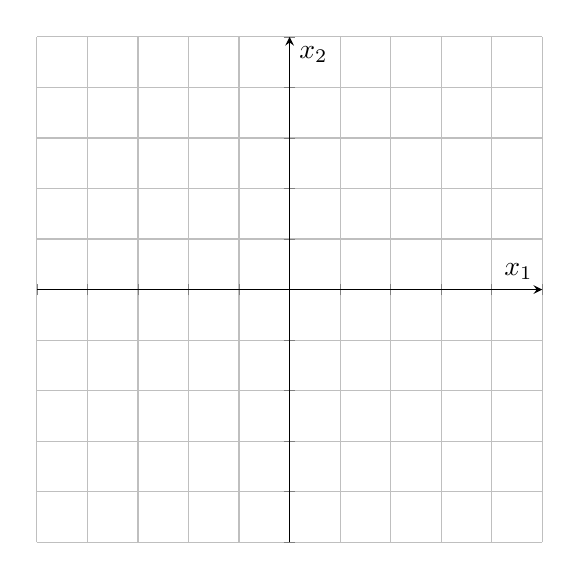
\begin{tikzpicture}
		\begin{axis}[
			height=8cm,
			width=8cm,
			axis lines = middle,
			xmin=-5, xmax=5, ymin=-5, ymax=5,
			xtick distance=1, ytick distance=1,
			xticklabels={}, yticklabels={,,},
			xlabel=\(x_1\), ylabel=\(x_2\),
			grid=major
		]
		\end{axis}
	\end{tikzpicture}
	\caption{Place (2.) here.}
\end{figure}
	\item Come up with a 3-by-2 matrix \(A\) that causes \(A\vec{x} = \vec{0}\) to \emph{only} have have the trivial solution.
	\item Is the solution set of the equation \(A\vec{x} = \vec{0}\) and \(A\vec{x} = \vec{b} \ne \vec{0}\) (where \(A\) is a matrix) always parallel to each other
		when sketched out? When is this true, and when is it not?
\end{enumerate}
\end{newquestion}

\section{Solutions}

\subsection{Solutions to Possible/Impossible Questions}
	\begin{table}[!h]
		\centering
		\begin{tabular}{c@{\hspace{2.5em}}cp{0.75\textwidth}}
			possible & impossible & \\
			\specialrule{\lightrulewidth}{0.25em}{1.25em}
			\bubble & \dbubble & A matrix \(A \in \mathbb{R}^{m \times 2}\) whose solution set for the equation \(A\vec{x} = \vec{b}\) is the \(x_2\)
						       axis, and \(\vec{b} \ne \vec{0}\). \\[0.75em]
			\dbubble & \bubble & A matrix \(A \in\mathbb{R}^{m\times n}\) and the solution set of \(A\vec{x} = \vec{0}\) is \(\mathbb{R}^{n}\).\\[0.75em]
			\bubble & \dbubble & A matrix \(A\in\mathbb{R}^{m\times n}\) such that the solution set of the equation \(A\vec{x}=\vec{0}\) is empty.\\[0.75em]
			\dbubble & \bubble & A solution \(\vec{v}\) to the equation \(A \vec{v} = \vec{0}\) but none of the entries of \(\vec{v}\) is 0. \\[0.75em]
			\bubble & \dbubble & A matrix \(A\in\mathbb{R}^{2\times 3}\) where \(\vec{0}\) is the only solution to the equation \(A\vec{x}=\vec{0}\).\\[0.75em]
			\bottomrule
		\end{tabular}
	\end{table}

\subsection{Solutions to Short Answer Questions}
\begin{enumerate}
	\item \(\vec{x} = \begin{bmatrix}0 \\ 1\end{bmatrix}\) has to be a solution to \(A\vec{x} = \vec{0}\). Recall that 
		\[A\vec{x} = 0 \iff \vec{a}_1x_1 + \vec{a}_2 = \vec{0}.\] Set \(x_1 = 0\) and \(x_1 = 1\). We get that 
		\[(0)\vec{a}_1 + (1)\vec{a}_2 = \vec{0}.\]
		We see that the first column is therefore \emph{anything} and the second column is the zero vector. As you encounter more and more of these types of 
		questions, you'll start to do this \emph{instinctively}.

	\item The paramteric vector form for the solution set of the inhomogeouns equation is 
		\[\vec{x} = \begin{bmatrix}0 \\ 1/2\end{bmatrix} + t\begin{bmatrix}-3 \\ 1\end{bmatrix}, \quad t \in \mathbb{R}.\footnote{A lot of people got the
		paramterization \(\vec{x} = \begin{bmatrix}3/2 \\ 0\end{bmatrix} + t\begin{bmatrix}-3 \\ 1 \end{bmatrix}\). Don't panic! Both answers
		are correct. Remember, \(\vec{v}_p\) is \emph{one} of many particular solutions. If you have any questions on this, please create a post on Piazza.}\]
		The sketch would look like this.
		(Also, the graph for the solution set to the homogenous equation is shown as well. Note that the red line is translated
		up by a half, that's the \(\vec{v}_p\) in \(\vec{x} = \vec{v}_p + \vec{v}_n\)!)
		\begin{figure}[!h]
			\centering
			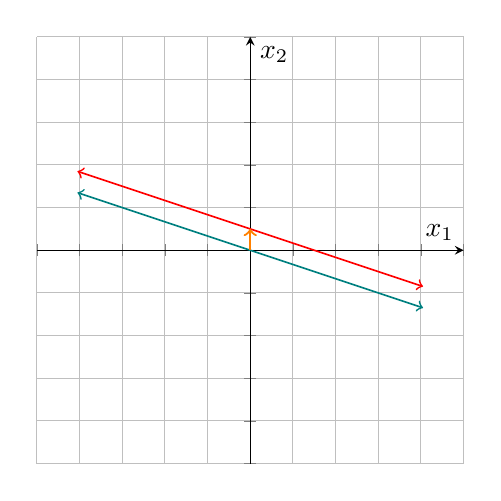
\begin{tikzpicture}
				\begin{axis}[
					height=7cm,
					width=7cm,
					axis lines = middle,
					xmin=-5, xmax=5, ymin=-5, ymax=5,
					xtick distance=1, ytick distance=1,
					xticklabels={}, yticklabels={,,},
					xlabel=\(x_1\), ylabel=\(x_2\),
					grid=major
				]
					\addplot[<->, red, semithick, domain=-1.35:1.35] ({-3 * x}, {0.5 + x});
					\addplot[<->, teal, semithick, domain=-1.35:1.35] ({-3 * x}, {x});
					\draw[->, orange, thick] (axis cs: 0, 0) -- (axis cs: 0, 0.5);
				\end{axis}
			\end{tikzpicture}
		\end{figure}

	\item We get a nontrivial solution once there is a free variable in the system corresponding to \(A\vec{x} = \vec{0}\). In order to ensure that the only solution is the
		trivial solution, find a 3-by-2 matrix that has \emph{no} free variables.
	
	\item Consider the case where the inhomogenous system is inconsistent.
\end{enumerate}
\end{document}